
\chapter{MATHEMATICAL BACKGROUND}

This chapter introduces the mathematical foundations of the methods studied in this work. Section~\ref{sec:boussinesq} presents the Boussinesq system and the limiting wave-equation regime. Section~\ref{sec:pseudospectral} develops the pseudospectral numerical method used to generate reference solutions. Sections~\ref{sec:neural_networks} and~\ref{sec:neural_operators} introduce, respectively, the neural network and neural operator architectures studied in this work.

% ---------------------------------------------------------------
\section{The Boussinesq System}
\label{sec:boussinesq}

The Boussinesq system is a model for long nonlinear dispersive waves in shallow water, governing the coupled evolution of two scalar fields: the free surface elevation $\eta(x,t)$ and the depth-averaged horizontal velocity $u(x,t)$, both depending on position $x$ and time $t$. In the one-dimensional, spatially periodic setting studied in this work, the system reads:
\begin{align}
    \eta_t + u_x + \alpha\, (\eta u)_x &= 0, \label{eq:bou1} \\
    u_t - \frac{\beta}{3}\, u_{xxt} + \eta_x + \alpha\, u u_x &= 0, \label{eq:bou2}
\end{align}
\noindent where $\alpha \geq 0$ is the nonlinearity parameter, controlling the magnitude of the convective coupling terms, and $\beta > 0$ is the dispersion parameter, governing the strength of the third-order correction $u_{xxt}$. This nondimensional form follows equation~(3.1) of \textcite{martins2023} (see also \textcite{martins2024}).

We note that $u u_x = \frac{1}{2}(u^2)_x$, so equation~\eqref{eq:bou2} can equivalently be written with the conservative flux $\frac{\alpha}{2}(u^2)_x$ in place of $\alpha\, u u_x$. Both forms appear in the implementations: the PINN residual uses $u u_x$ directly via automatic differentiation, while the pseudospectral solver exploits $\frac{1}{2}(u^2)_x$ for the physical-space product, as detailed in Section~\ref{sec:pseudospectral}.

The system is studied on the periodic domain $\Omega = [-L, L]$ with initial conditions:
\begin{equation}\label{eq:ic}
    \eta(x, 0) = A\,\operatorname{sech}^2(x), \qquad u(x, 0) = 0,
\end{equation}
\noindent where $A > 0$ is the initial amplitude, $L > 0$ is the domain half-length, and $\operatorname{sech}(z) = \frac{2}{e^z + e^{-z}}$ is the hyperbolic secant. This profile places a solitary-wave-like crest at the center $x = 0$ with zero initial velocity.

\begin{figure}[h!]
    \centering
    
\includegraphics[width=0.72\textwidth]{soliton_profile.png}
    \caption{Initial condition $\eta(x,0) = A\operatorname{sech}^2(x)$ for $A = 1$.}
    \label{fig:soliton_profile}
    \autoriapropria
\end{figure}

\subsection{Recovering the Wave Equation}
\label{subsec:wave_eq}

In the doubly linear limit $\alpha = \beta = 0$, all nonlinear and dispersive terms vanish and the Boussinesq system reduces to the symmetric hyperbolic system:
\begin{align}
    \eta_t + u_x &= 0, \label{eq:wave1} \\
    u_t + \eta_x &= 0. \label{eq:wave2}
\end{align}
To obtain a single scalar equation, differentiate~\eqref{eq:wave1} with respect to $t$:
\begin{equation}
    \eta_{tt} + u_{xt} = 0.
\end{equation}
Differentiate~\eqref{eq:wave2} with respect to $x$:
\begin{equation}
    u_{tx} + \eta_{xx} = 0.
\end{equation}
Since $u_{xt} = u_{tx}$, subtracting the second from the first yields the wave equation for $\eta$:
\begin{equation}\label{eq:wave_eq}
    \eta_{tt} = \eta_{xx},
\end{equation}
and the reverse procedure gives the same equation for $u$.

D'Alembert's formula \parencite{debnath2012} provides the general solution to~\eqref{eq:wave_eq}. Given initial data
\begin{equation}
    \eta(x, 0) = f(x), \qquad \eta_t(x, 0) = g(x),
\end{equation}
the solution is:
\begin{equation}\label{eq:dalembert}
    \eta(x,t) = \frac{f(x+t) + f(x-t)}{2}
            + \frac{1}{2}\int_{x-t}^{x+t} g(s)\,ds.
\end{equation}

We now apply this to the initial conditions~\eqref{eq:ic}. From~\eqref{eq:wave1}, $\eta_t(x,0) = -u_x(x,0) = 0$, so:
\begin{equation}
    f(x) = A\operatorname{sech}^2(x), \qquad g(x) = 0.
\end{equation}
Since $g \equiv 0$, the integral in~\eqref{eq:dalembert} vanishes and the surface elevation evolves as:
\begin{equation}\label{eq:dalembert_eta}
    \eta(x, t) = \frac{A}{2}\bigl[\operatorname{sech}^2(x+t) + \operatorname{sech}^2(x-t)\bigr].
\end{equation}
For $u$, from~\eqref{eq:wave2} we have $u_t(x,0) = -\eta_x(x,0)$, giving:
\begin{equation}
    f(x) = 0, \qquad g(x) = -\eta_x(x,0).
\end{equation}
The $f = 0$ term vanishes in~\eqref{eq:dalembert}, leaving:
\begin{equation}
    u(x,t) = \frac{1}{2}\int_{x-t}^{x+t} \bigl(-\eta_x(s,0)\bigr)\,ds
            = -\frac{1}{2}\bigl[\eta(x+t,0) - \eta(x-t,0)\bigr].
\end{equation}
Substituting $\eta(x,0) = A\operatorname{sech}^2(x)$:
\begin{equation}\label{eq:dalembert_u}
    u(x,t) = \frac{A}{2}\bigl[\operatorname{sech}^2(x-t) - \operatorname{sech}^2(x+t)\bigr].
\end{equation}
The initial bump of amplitude $A$ splits into two counter-propagating pulses of amplitude $A/2$, traveling at speed $\pm 1$ without changing shape. Any deviation from this wave-equation baseline in the full system~\eqref{eq:bou1}--\eqref{eq:bou2} is attributable either to dispersion ($\beta > 0$) or to nonlinearity ($\alpha > 0$).

% ---------------------------------------------------------------
\section{Pseudospectral Method}
\label{sec:pseudospectral}

The pseudospectral method exploits two complementary representations of the solution: Fourier space, where derivatives become exact algebraic multiplications, and physical space, where pointwise nonlinear operations are inexpensive. By alternating between the two representations as needed, the method attains spectral accuracy in space while handling the nonlinear coupling efficiently.

\subsection{Spatial Discretization and the Discrete Fourier Transform}
\label{subsec:dft}

The spatial domain $\Omega = [-L, L]$ of total length $2L$ is discretized into $N_x$ equispaced points:
\begin{equation}
    x_j = -L + j\,\Delta x, \qquad \Delta x = \frac{2L}{N_x},
    \qquad j = 0, \ldots, N_x - 1.
\end{equation}
The Discrete Fourier Transform (DFT) of a function $f$ sampled at these points is \parencite{trefethen2000}:
\begin{equation}\label{eq:dft}
    \hat{f}(k) = \sum_{j=0}^{N_x-1} f(x_j)\, e^{-2\pi i k j / N_x},
    \qquad k = -\tfrac{N_x}{2}, \ldots, \tfrac{N_x}{2} - 1,
\end{equation}
with its inverse recovering the physical values:
\begin{equation}\label{eq:idft}
    f(x_j) = \frac{1}{N_x} \sum_{k} \hat{f}(k)\, e^{2\pi i k j / N_x}.
\end{equation}
The fundamental identity of the DFT with respect to differentiation is that, for a periodic function, the spatial derivative transforms into a pointwise multiplication \parencite{trefethen2000, engsigkarup2012}:
\begin{equation}\label{eq:dft_deriv_raw}
    \widehat{(f_x)}(k) = i \frac{\pi k}{L}\, \hat{f}(k), \quad
    \widehat{(f_{xx})}(k) = -\frac{\pi^2 k^2}{L^2}\, \hat{f}(k).
\end{equation}
This is in contrast to finite-difference methods, where derivatives are approximated with truncation error; in the DFT, equation~\eqref{eq:dft_deriv_raw} is exact for periodic functions.

We define the wavenumber of mode $k$ on $[-L,L]$ as:
\begin{equation}\label{eq:xi_def}
    \xi_k \;:=\; \frac{\pi k}{L}.
\end{equation}
With this definition, the derivative identities read:
\begin{equation}\label{eq:dft_deriv}
    \widehat{(f_x)}(k) = i\,\xi_k\,\hat{f}(k), \qquad
    \widehat{(f_{xx})}(k) = -\xi_k^2\,\hat{f}(k).
\end{equation}

\subsection{Spectral Formulation of the Boussinesq System}
\label{subsec:spectral_bou}

To bring the Boussinesq system~\eqref{eq:bou1}--\eqref{eq:bou2} into the Fourier domain \parencite{martins2023}, we apply the DFT to each equation and use the derivative identities~\eqref{eq:dft_deriv}. The first equation, treating $\widehat{(\eta u)}(k,t)$ as a given nonlinear term, becomes:
\begin{equation}\label{eq:eta_t_spectral}
    \hat{\eta}_t(k,t) = -i\,\xi_k\,\hat{u}(k,t)
    - \alpha\, i\,\xi_k\,\widehat{(\eta u)}(k,t).
\end{equation}
The second equation requires more care because of the $u_{xxt}$ term. Since spatial derivatives commute with the DFT:
\begin{equation}
    \widehat{(u_{xxt})}(k,t) = -\xi_k^2\,\hat{u}_t(k,t).
\end{equation}
Substituting into the DFT of~\eqref{eq:bou2}:
\begin{equation}
    \hat{u}_t(k,t) + \frac{\beta}{3}\,\xi_k^2\,\hat{u}_t(k,t)
    + i\,\xi_k\,\hat{\eta}(k,t)
    + \alpha\, i\,\xi_k\,\widehat{\!\left(\tfrac{1}{2}u^2\right)}(k,t) = 0.
\end{equation}
Collecting the $\hat{u}_t(k,t)$ terms on the left and solving algebraically:
\begin{equation}\label{eq:u_t_spectral}
    \hat{u}_t(k,t) = \frac{
        -i\,\xi_k\,\hat{\eta}(k,t)
        - \alpha\, i\,\xi_k\,\widehat{\!\left(\tfrac{1}{2}u^2\right)}(k,t)
    }{
        1 + \dfrac{\beta\,\xi_k^2}{3}
    }.
\end{equation}
The operator $1 - \frac{\beta}{3}\frac{\partial^2}{\partial x^2}$, which requires a linear solve in physical space, becomes the diagonal scalar $1 + \frac{\beta\,\xi_k^2}{3}$ in Fourier space, reducing its inversion to a single division per mode.

The nonlinear terms $\widehat{(\eta u)}(k,t)$ and $\widehat{(\frac{1}{2}u^2)}(k,t)$ cannot be computed directly in Fourier space without a convolution sum, which costs $O(N_x^2)$. The pseudospectral approach avoids this by computing products in physical space. For $\widehat{(\eta u)}(k,t)$, the procedure is:
\begin{enumerate}
    \item recover $\eta(x_j)$ and $u(x_j)$ by applying the inverse DFT~\eqref{eq:idft};
    \item compute the product $(\eta u)_j = \eta(x_j)\cdot u(x_j)$ pointwise on the grid;
    \item apply the DFT~\eqref{eq:dft} to obtain $\widehat{(\eta u)}(k,t)$.
\end{enumerate}
Similarly, $\widehat{(\frac{1}{2}u^2)}(k,t)$ is obtained by squaring $u(x_j)$ pointwise and transforming. Since each DFT/IDFT costs $O(N_x \log N_x)$ via the Fast Fourier Transform (FFT), this pseudospectral strategy assembles each nonlinear term in $O(N_x \log N_x)$ rather than $O(N_x^2)$.

\subsection{Time Evolution via Runge-Kutta 4}
\label{subsec:rk4}

We define the pseudospectral right-hand side operator $F$ as the map
\begin{equation}\label{eq:rhs_F}
    F\!\left(\hat{\eta},\hat{u}\right)(k)
    \;=\;
    \begin{pmatrix}
        -i\,\xi_k\,\hat{u}(k)
        - \alpha\,i\,\xi_k\,\widehat{(\eta u)}(k) \\[6pt]
        \dfrac{
            -i\,\xi_k\,\hat{\eta}(k)
            - \alpha\,i\,\xi_k\,\widehat{\!\left(\tfrac{1}{2}u^2\right)}\!(k)
        }{
            1 + \dfrac{\beta\,\xi_k^2}{3}
        }
    \end{pmatrix},
\end{equation}
so that $F(\hat{\eta},\hat{u}) = \bigl(\hat{\eta}_t,\, \hat{u}_t\bigr)$ as given by equations~\eqref{eq:eta_t_spectral}--\eqref{eq:u_t_spectral}, with nonlinear terms assembled by the pseudospectral procedure above. Time evolution uses the classical fourth-order Runge-Kutta (RK4) scheme. Given the spectral state $y_n = (\hat{\eta}^n, \hat{u}^n)$ at time $t_n$, the four stage evaluations $\kappa_1, \kappa_2, \kappa_3, \kappa_4$ and the update to $t_{n+1} = t_n + \Delta t$ are:
\begin{align}
    \kappa_1 &= F(y_n), \nonumber \\
    \kappa_2 &= F\!\left(y_n + \tfrac{\Delta t}{2}\, \kappa_1\right), \nonumber \\
    \kappa_3 &= F\!\left(y_n + \tfrac{\Delta t}{2}\, \kappa_2\right), \nonumber \\
    \kappa_4 &= F\!\left(y_n + \Delta t\, \kappa_3\right), \nonumber \\
    y_{n+1}  &= y_n + \frac{\Delta t}{6}\,(\kappa_1 + 2\,\kappa_2 + 2\,\kappa_3 + \kappa_4).
    \label{eq:rk4}
\end{align}
At each stage, the intermediate state is decoded to physical space to assemble the nonlinear products, then encoded back to Fourier space to evaluate the spectral derivatives. This split between physical-space products and Fourier-space derivatives is the defining operation of the pseudospectral method.

% ---------------------------------------------------------------
\subsection{Training Dataset}
\label{sec:dataset}

The numerical experiments in this work vary only the PDE parameters $(\alpha,\beta)$ while keeping the initial condition fixed at~\eqref{eq:ic}. The models are therefore trained and evaluated on the dataset
\begin{equation}\label{eq:dataset}
    \mathcal{D} = \bigl\{\bigl((\alpha_i,\beta_i),\,(\eta_i,u_i)\bigr)\bigr\}_{i=1}^{M},
\end{equation}
where $(\alpha_i,\beta_i)$ are the nonlinearity and dispersion parameters for the $i$-th sample, and $(\eta_i,u_i)$ is the corresponding space-time solution obtained from the pseudospectral solver of Section~\ref{sec:pseudospectral} with those parameters and the shared initial condition~\eqref{eq:ic}.

% ---------------------------------------------------------------
\section{Neural Networks}
\label{sec:neural_networks}

This section introduces the neural network architectures central to this work: Multilayer Perceptrons as the building block, Physics-Informed Neural Networks as the first SciML method studied, and the Neural Tangent Kernel framework that provides the theoretical explanation for the spectral bias phenomenon.

\subsection{Multilayer Perceptrons}
\label{subsec:mlp}

In this work, we focus on Multilayer Perceptrons (MLPs), popularized by \textcite{rumelhart1986}. These networks are compositions of affine transformations parametrized by tunable weights and biases, separated by nonlinear activations, where an optimization process fits the network to a dataset.

Given a labeled dataset ${\{(x_i, u_i)\}}_{i=1}^{N_{\mathrm{data}}}$, the objective is to fit the function $u_{\theta}(x)$ by minimizing a loss function, typically the Mean Squared Error (MSE). With $\|\cdot\|$ denoting the Euclidean norm, the unconstrained optimization problem is:
\begin{equation}
    \text{MSE}(\theta) = \frac{1}{N_{\mathrm{data}}} \sum_{i=1}^{N_{\mathrm{data}}} \| u_{\theta}(x_i) - u_i \|^2. \label{eq:data_loss_nn}
\end{equation}
The MLP $u_\theta: \mathbb{R}^{d_{\mathrm{in}}} \to \mathbb{R}^{d_{\mathrm{out}}}$ is defined by the composition:
\begin{align}
    h^{(0)}       &= x \in \mathbb{R}^{d_{\mathrm{in}}}, \label{eq:input}                                                                 \\
    h^{(l)}       &= \sigma \left( W^{(l)} h^{(l-1)} + b^{(l)} \right) \in \mathbb{R}^{N},
                   \quad l = 1, \dots, L-1, \label{eq:hidden} \\
    u_{\theta}(x) &= W^{(L)} h^{(L-1)} + b^{(L)} \in \mathbb{R}^{d_{\mathrm{out}}}. \label{eq:output}
\end{align}
\noindent where:
\begin{itemize}
    \item $L \in \mathbb{N}$ is the number of layers and $N \in \mathbb{N}$ the number of neurons per hidden layer;
    \item $W^{(l)} \in \mathbb{R}^{N \times N}$ and $b^{(l)} \in \mathbb{R}^N$ are the weight matrix and bias vector at layer $l$, with $W^{(1)} \in \mathbb{R}^{d_{\mathrm{in}} \times N}$ and $W^{(L)} \in \mathbb{R}^{N \times d_{\mathrm{out}}}$ adapted at the boundaries;
    \item $\sigma : \mathbb{R} \to \mathbb{R}$ is a sigmoidal activation function applied elementwise, satisfying $\sigma(t) \to 1$ as $t \to +\infty$ and $\sigma(t) \to 0$ as $t \to -\infty$;
    \item $\theta = \{W^{(l)}, b^{(l)}\}_{l=1}^{L}$ denotes all trainable parameters.
\end{itemize}

If the activation function is sigmoidal, MLPs are universal approximators: they can approximate any continuous function on a compact domain to arbitrary precision \parencite{cybenko1989}.

In Figure~\ref{fig:MLP_depiction}, we show a common depiction of the neural network. Here the input vector is the pair $(x,t) \in \mathbb{R}^2$ and the output is $(\eta_{\theta}(x,t), u_{\theta}(x,t)) \in \mathbb{R}^2$.

\begin{figure}[h!]
    \centering
    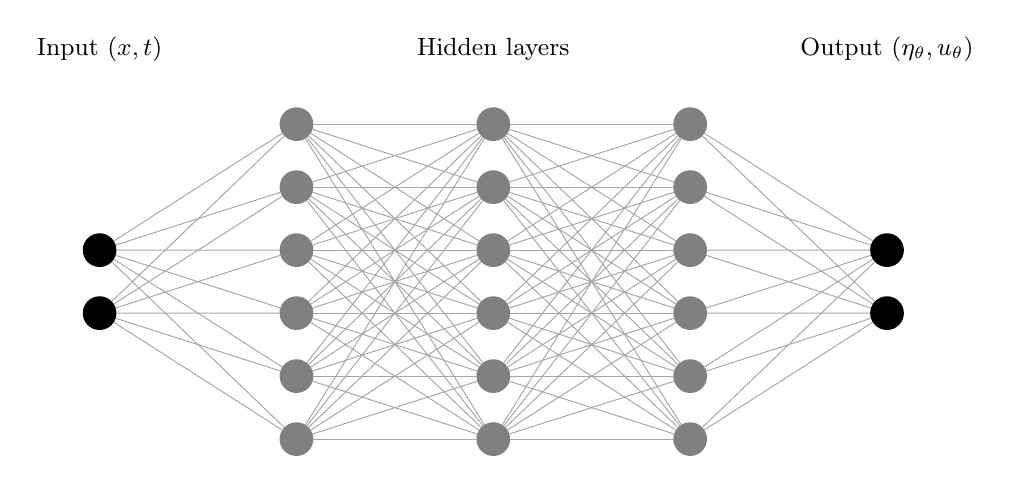
\begin{tikzpicture}[
            x=1cm,
            y=1cm,
            nnnode/.style={circle, draw, line width=0.8pt, minimum size=0.40cm, inner sep=0pt},
            inout/.style={nnnode, fill=black, draw=black},
            hidden/.style={nnnode, fill=gray, draw=gray},
            conn/.style={draw=gray!70, line width=0.35pt}
        ]
        \node[inout] (x1) at (0,-2.4) {};
        \node[inout] (x2) at (0,-3.2) {};
        \node at (0,0.15) {\small Input $(x,t)$};
        \foreach \i in {1,...,6} { \node[hidden] (h1_\i) at (2.5,-0.8*\i) {}; }
        \foreach \i in {1,...,6} { \node[hidden] (h2_\i) at (5.0,-0.8*\i) {}; }
        \node at (5.0,0.15) {\small Hidden layers};
        \foreach \i in {1,...,6} { \node[hidden] (h3_\i) at (7.5,-0.8*\i) {}; }
        \node[inout] (out1) at (10.0,-2.4) {};
        \node[inout] (out2) at (10.0,-3.2) {};
        \node at (10.0,0.15) {\small Output $(\eta_{\theta}, u_{\theta})$};
        \foreach \j in {1,...,6} {
            \draw[conn] (x1) -- (h1_\j);
            \draw[conn] (x2) -- (h1_\j);
        }
        \foreach \i in {1,...,6} {
            \foreach \j in {1,...,6} {
                \draw[conn] (h1_\i) -- (h2_\j);
                \draw[conn] (h2_\i) -- (h3_\j);
            }
        }
        \foreach \i in {1,...,6} {
            \draw[conn] (h3_\i) -- (out1);
            \draw[conn] (h3_\i) -- (out2);
        }
    \end{tikzpicture}
    \caption{Example of MLP architecture of input $(x, t)$, with $L=3$ hidden layers and $N=6$ neurons per layer.}
    \label{fig:MLP_depiction}
    \autoriapropria
\end{figure}

\subsection{Physics-Informed Neural Networks}
\label{subsec:pinn}

Introduced by \textcite{raissi2017}, Physics-Informed Neural Networks (PINNs) insert the PDE directly into the optimization process, forcing the neural network to satisfy the model equations and approximating the PDE solution.

Consider the general PDE Initial Value Problem:
\begin{equation}\label{eq:generic_pde}
    \left\{
    \begin{aligned}
        \mathcal{D}[u](x,t) &= 0, \quad \forall (x,t) \in \Omega \times (0,T], \\
        u(x,0)              &= u_0(x), \quad x \in \Omega,
    \end{aligned}
    \right.
\end{equation}
\noindent where $\mathcal{D}$ is a differential operator on $u$, $\Omega \times (0,T]$ is the spatio-temporal domain, and $u_0$ is the initial condition.

The PDE residual loss penalizes violation of the governing equation at collocation points $\{(x_i,t_i)\}_{i=1}^{N_\mathcal{D}} \subset \Omega \times (0,T]$:
\begin{equation}
    \text{MSE}_\mathcal{D}(\theta) = \frac{1}{N_\mathcal{D}}\sum_{i=1}^{N_\mathcal{D}}
    \left\| \mathcal{D}[u_\theta](x_i,t_i)\right\|^2.
\end{equation}
The initial condition is enforced at collocation points $\{x_i\}_{i=1}^{N_0} \subset \Omega$:
\begin{equation}
    \text{MSE}_0(\theta) = \frac{1}{N_0}\sum_{i=1}^{N_0}
    \left\| u_\theta(x_i,0) - u_0(x_i) \right\|^2.
\end{equation}
The combined PINN loss is:
\begin{equation}\label{eq:loss_pinn}
    \mathcal{L}(\theta) = \text{MSE}_\mathcal{D}(\theta) + \text{MSE}_0(\theta).
\end{equation}

Due to the compositional structure of MLPs, PINN implementations evaluate PDE residuals via Automatic Differentiation (AD) \parencite{linnainmaa1970, paszke2019pytorch}, using ADAM \parencite{kingma2014adam} or L-BFGS \parencite{nocedal1980lbfgs} as the optimizer.

\subsubsection{Application to the Boussinesq Dataset}
\label{subsubsec:pinn_loss_boussinesq}

For the Boussinesq system, a separate PINN is trained for each sample $(\alpha_i,\beta_i) \in \mathcal{D}$~\eqref{eq:dataset}. The differential operator $\mathcal{D}$ in the generic problem~\eqref{eq:generic_pde} is instantiated as the pair of Boussinesq residuals with fixed parameters $(\alpha_i,\beta_i)$:
\begin{align}
    \mathcal{D}_1[u_\theta] &= (\eta_\theta)_t + (u_\theta)_x + \alpha_i\,\bigl((\eta_\theta\,u_\theta)_x\bigr), \\
    \mathcal{D}_2[u_\theta] &= (u_\theta)_t - \tfrac{\beta_i}{3}(u_\theta)_{xxt} + (\eta_\theta)_x + \alpha_i\,(u_\theta(u_\theta)_x).
\end{align}
The combined loss~\eqref{eq:loss_pinn} for sample $i$ then reads:
\begin{equation}\label{eq:pinn_loss_boussinesq}
    \mathcal{L}_i(\theta) = \frac{1}{N_\mathcal{D}}\sum_{l=1}^{N_\mathcal{D}}
    \Bigl[\mathcal{D}_1[u_\theta](x_l,t_l)^2 + \mathcal{D}_2[u_\theta](x_l,t_l)^2\Bigr]
    + \frac{1}{N_0}\sum_{l=1}^{N_0}
    \Bigl[(\eta_\theta(x_l,0)-\eta_0(x_l))^2 + (u_\theta(x_l,0)-u_0(x_l))^2\Bigr],
\end{equation}
where $\eta_0$ and $u_0$ are given by the shared initial condition~\eqref{eq:ic}. Because the parameters $(\alpha_i,\beta_i)$ enter the residuals explicitly, each PINN encodes knowledge of a single sample and must be retrained for every new parameter pair.

\subsection{Neural Tangent Kernel}
\label{subsec:ntk}

To understand how the PINN loss is minimized, consider gradient descent with learning rate $\lambda > 0$:
\begin{equation}\label{eq:gd_discrete}
    \theta_{k+1} = \theta_k - \lambda\,\nabla_\theta\mathcal{L}(\theta_k).
\end{equation}
Introducing a continuous training-time variable $\tau = k\lambda$ and taking the limit $\lambda \to 0$ converts the discrete iteration to the gradient flow ODE:
\begin{equation}\label{eq:grad_flow}
    \frac{d\theta}{d\tau} = -\nabla_\theta \mathcal{L}(\theta).
\end{equation}
For the IVP~\eqref{eq:generic_pde}, the PINN enforces $N_0$ initial-condition constraints and $N_\mathcal{D}$ PDE-residual constraints. Group all residuals into a single error vector:
\begin{equation}\label{eq:error_vector}
    e(\theta) =
    \begin{bmatrix}
        u_\theta(x_1,0) - u_0(x_1) \\
        \vdots \\
        u_\theta(x_{N_0},0) - u_0(x_{N_0}) \\[3pt]
        \mathcal{D}[u_\theta](x_1,t_1) \\
        \vdots \\
        \mathcal{D}[u_\theta](x_{N_\mathcal{D}},t_{N_\mathcal{D}})
    \end{bmatrix}
    \in \mathbb{R}^{N_r},
    \qquad N_r = N_0 + N_\mathcal{D}.
\end{equation}
The PINN loss is half the squared norm of this vector:
\begin{equation}\label{eq:loss_quadratic}
    \mathcal{L}(\theta) = \frac{1}{2}\,\|e(\theta)\|^2.
\end{equation}
Define the Jacobian of residuals with respect to parameters:
\begin{equation}\label{eq:jacobian}
    J(\theta) = \frac{\partial e}{\partial\theta} \in \mathbb{R}^{N_r \times N_\theta},
    \qquad J_{ij} = \frac{\partial e_i}{\partial\theta_j},\quad i = 1,\ldots,N_r,\; j = 1,\ldots,N_\theta,
\end{equation}
where $N_\theta$ is the total number of trainable parameters. The matrix $J$ has $N_r$ rows, one per constraint point, and $N_\theta$ columns, one per parameter; each row $J_i \in \mathbb{R}^{N_\theta}$ is the parameter-gradient of the $i$-th residual. Since $\mathcal{L} = \tfrac{1}{2}\|e\|^2 = \tfrac{1}{2}\sum_i e_i^2$, the $j$-th component of the gradient is
\begin{equation}
    \frac{\partial \mathcal{L}}{\partial \theta_j}
    = \sum_{i=1}^{N_r} e_i(\theta)\,\frac{\partial e_i}{\partial \theta_j}
    = \sum_{i=1}^{N_r} J_{ij}\,e_i(\theta).
\end{equation}
Collecting all $j$ into a column vector gives:
\begin{equation}\label{eq:loss_grad}
    \nabla_\theta\mathcal{L} = J(\theta)^T\,e(\theta) \in \mathbb{R}^{N_\theta}.
\end{equation}
Substituting into the gradient flow~\eqref{eq:grad_flow}:
\begin{equation}\label{eq:param_dynamics}
    \frac{d\theta}{d\tau} = -J(\theta)^T\,e(\tau).
\end{equation}
To find how the residual vector itself evolves, differentiate $e_i(\theta(\tau))$ with respect to $\tau$ via the chain rule:
\begin{equation}
    \frac{de_i}{d\tau}
    = \sum_{j=1}^{N_\theta} \frac{\partial e_i}{\partial \theta_j}\,\frac{d\theta_j}{d\tau}
    = J_i(\theta)\cdot\frac{d\theta}{d\tau}.
\end{equation}
Stacking over all $i = 1,\ldots,N_r$:
\begin{equation}
    \frac{de}{d\tau} = J(\theta)\,\frac{d\theta}{d\tau}.
\end{equation}
Substituting~\eqref{eq:param_dynamics}:
\begin{equation}\label{eq:ntk_dynamics}
    \frac{de}{d\tau}
    = J(\theta)\bigl(-J(\theta)^T e(\tau)\bigr)
    = -\underbrace{J(\theta)\,J(\theta)^T}_{K(\theta)\;\in\;\mathbb{R}^{N_r\times N_r}}\,e(\tau).
\end{equation}
The matrix $K(\theta) = J(\theta)J(\theta)^T$ is the empirical Neural Tangent Kernel (NTK) \parencite{jacot2018}. It is symmetric positive semi-definite by construction ($v^T K v = \|J^T v\|^2 \geq 0$ for every $v$).

\subsection{Spectral Bias}
\label{subsec:spectral_bias}

The spectral bias (or frequency principle) is the empirical observation that neural networks trained by gradient-based methods learn low-frequency components of the target function significantly faster than high-frequency ones \parencite{rahaman2019}.

For a network with a sufficiently large number of parameters, the Jacobian $J(\theta)$ changes negligibly during training \parencite{jacot2018, wang2022ntk}. In this regime $K(\theta(\tau)) \approx K_0 = J_0 J_0^T$, and equation~\eqref{eq:ntk_dynamics} becomes a linear ODE with constant coefficients:
\begin{equation}\label{eq:error_linear_ode}
    \frac{de}{d\tau} = -K_0\,e(\tau), \qquad e(0) = e_0,
\end{equation}
with solution $e(\tau) = e^{-K_0 \tau}\,e_0$. Since $K_0 \in \mathbb{R}^{N_r \times N_r}$ is symmetric positive semi-definite, it diagonalizes as $K_0 = V\Lambda V^T$, where $V \in \mathbb{R}^{N_r \times N_r}$ is orthogonal and $\Lambda = \mathrm{diag}(\lambda_1, \ldots, \lambda_{N_r})$ with $\lambda_k \geq 0$. Expanding the initial error in the eigenbasis $e_0 = \sum_k c_k^{(0)} v_k$ decouples~\eqref{eq:error_linear_ode} into $N_r$ independent scalar ODEs:
\begin{equation}\label{eq:error_mode}
    \frac{dc_k}{d\tau} = -\lambda_k\,c_k \;\implies\; c_k(\tau) = c_k(0)\,e^{-\lambda_k \tau},
\end{equation}
giving the full error evolution:
\begin{equation}
    e(\tau) = \sum_{k=1}^{N_r} c_k(0)\,e^{-\lambda_k \tau}\,v_k.
\end{equation}
Each error mode $v_k$ decays at its own exponential rate $\lambda_k$: modes with large eigenvalues are suppressed quickly, while modes with small eigenvalues persist throughout training.

The NTK analysis explains why this affects high frequencies preferentially. Recall that $K_0 = J_0 J_0^T$, so $K_{0,ij} = J_{0,i} \cdot J_{0,j}$, where each row $J_{0,i} = \nabla_\theta e_i(\theta_0) \in \mathbb{R}^{N_\theta}$ is the parameter-gradient of residual $e_i$ evaluated at spatial location $x_i$. Since $u_\theta$ is a composition of smooth activations applied to affine maps, the map $x_i \mapsto J_{0,i}$ is itself smooth: nearby collocation points have similar gradient directions. Consequently, the kernel entries $K_{0,ij} = J_{0,i} \cdot J_{0,j}$ vary slowly as a function of $(x_i, x_j)$, and a slowly-varying kernel cannot efficiently represent rapidly oscillating eigenvectors. This implies the following chain:
\begin{enumerate}
    \item the rows of $J_0$ vary smoothly with the spatial location of the constraint point;
    \item the eigenvalues $\lambda_k$ of $K_0$ associated with high-frequency eigenvectors are systematically small;
    \item the corresponding error modes $c_k(\tau) = c_k(0)\,e^{-\lambda_k \tau}$ decay slowly.
\end{enumerate}
Gradient descent is consequently slow to correct high-frequency error components, regardless of the specific operator $\mathcal{D}$: spectral bias is a universal feature of PINNs applied to any IVP of the form~\eqref{eq:generic_pde} \parencite{rahaman2019, khodakarami2026}. This phenomenon will be clearly visible in the numerical results of Chapter~4.

\section{Neural Operators}
\label{sec:neural_operators}

Neural operators generalize neural networks from learning finite-dimensional mappings to learning operators between infinite-dimensional function spaces. This section introduces the general framework, then the Fourier Neural Operator (FNO) as the principal architecture, and finally the Physics-Informed Neural Operator (PINO) as the physics-constrained extension.

\subsection{General Definition}
\label{subsec:no_general}

Let $D \subset \mathbb{R}^{d}$ be a bounded open domain and let $\mathcal{A}(D; \mathbb{R}^{d_a})$ and $\mathcal{U}(D; \mathbb{R}^{d_u})$ be Banach spaces of functions \parencite{kreyszig1978introductory}. The target operator is a (potentially nonlinear) map
\begin{equation}
    G^\dagger : \mathcal{A} \to \mathcal{U},
    \qquad a \mapsto u = G^\dagger(a),
\end{equation}
where both the input $a$ and the output $u$ are functions defined on $D$.

In this work, $G^\dagger$ is the solution operator of the Boussinesq system: given a parameter encoding $(c, u_0)$ containing the PDE coefficients $(\alpha, \beta)$ and the initial condition $u_0$, the operator returns the full space-time solution $(\eta, u)$.

A neural operator $G_\theta$ approximates $G^\dagger$ by composing linear integral operators with pointwise nonlinearities. Each linear layer applies an operator of the form:
\begin{equation}
    (\mathcal{K} v)(x) = \int_{D} \kappa(x, y)\,v(y)\,dy,
\end{equation}
where $\kappa : D \times D \to \mathbb{R}^{d_u \times d_u}$ is a learned kernel. The full neural operator architecture stacks these integral layers into the composition:
\begin{equation}\label{eq:no_arch}
    G_\theta = Q \circ \sigma\Big(W_L + \mathcal{K}_L\Big) \circ \cdots \circ \sigma\Big(W_1 + \mathcal{K}_1\Big) \circ P,
\end{equation}
\noindent where:
\begin{itemize}
    \item $P : \mathbb{R}^{d_a} \to \mathbb{R}^{d_c}$ is the lifting operator, mapping the input $a(x)$ pointwise to a higher-dimensional channel representation with $d_c \gg d_a$;
    \item $\sigma\!\Big(W_\ell + \mathcal{K}_\ell\Big)$, for $\ell = 1, \ldots, L$, are the operator layers, each combining a local linear map $W_\ell$ with a nonlocal integral operator $\mathcal{K}_\ell$, followed by a pointwise activation $\sigma$;
    \item $Q : \mathbb{R}^{d_c} \to \mathbb{R}^{d_u}$ is the projection operator mapping the final channel representation back to the output dimension.
\end{itemize}
Different choices of kernel parametrization for each $\mathcal{K}_\ell$ give rise to different neural operator architectures.

\subsection{Fourier Neural Operators}
\label{subsec:fno}

Presented by \textcite{li2020fourier}, the Fourier Neural Operator (FNO) is the neural operator~\eqref{eq:no_arch} in which each $\mathcal{K}_\ell$ uses a shift-invariant kernel: $\kappa_\ell(x, y) = \kappa_\ell(x - y)$. This assumption turns each integral operator into a convolution, which by the convolution theorem can be evaluated efficiently in the frequency domain.

Each spectral layer updates the channel representation via:
\begin{equation}
    v_{\ell+1}(x) = \sigma \Big( (W_\ell\,v_\ell)(x) + (\mathcal{K}_\ell v_\ell)(x) \Big).
\end{equation}
The operator $\mathcal{K}_\ell$ acts via convolution with the shift-invariant kernel $\kappa_\ell$:
\begin{equation}
    (\mathcal{K}_\ell v_\ell)(x) = \int_{D} \kappa_\ell(x-y)\,v_\ell(y)\,dy.
\end{equation}
By the convolution theorem, this equals:
\begin{equation}
    (\mathcal{K}_\ell v_\ell)(x) = \mathcal{F}^{-1} \Big( \mathcal{F}(\kappa_\ell) \cdot \mathcal{F}(v_\ell) \Big)(x).
    \label{eq:fno_approximation}
\end{equation}
To see how this is parametrized, recall that for a periodic function $f$ on $[0, 2\pi]$:
\begin{equation}
    f(x) = \sum_{k \in \mathbb{Z}} \hat{f}(k) \, e^{ikx}, \qquad \hat{f}(k) = \frac{1}{2\pi} \int_0^{2\pi} f(x) e^{-ikx} \,dx.
\end{equation}
The convolution $(\kappa * v)$ simplifies to:
\begin{equation}
    (\kappa * v)(x) = \int_0^{2\pi} \kappa(x-y)\, v(y)\, dy
    = \sum_{k \in \mathbb{Z}} \bigl(2\pi\, \hat{\kappa}(k)\, \hat{v}(k)\bigr)\, e^{ikx}.
\end{equation}
Instead of learning $\kappa_\ell$ as a function in physical space, the FNO directly parametrizes its Fourier coefficients as learnable complex-valued matrices $R_{\ell,k} \approx 2\pi\,\hat{\kappa}_\ell(k)$. Only the $|k| \le k_{\max}$ low-frequency modes are retained, with all others set to zero; $k_{\max}$ is a hyperparameter.

\subsubsection{Training Objective}
\label{subsubsec:fno_loss}

The FNO is trained as a pure supervised learning problem. Given the dataset $\mathcal{D}$~\eqref{eq:dataset} of parameter-solution pairs, the training objective minimizes the mean squared error between the predicted and reference space-time fields:
\begin{equation}\label{eq:fno_loss}
    \mathcal{L}_{\text{FNO}} = \frac{1}{M}\sum_{i=1}^{M}\frac{1}{N_x N_t}\sum_{j=0}^{N_x-1}\sum_{n=0}^{N_t}
    \Bigl[(\eta_\theta^i(x_j,t_n) - \eta_i(x_j,t_n))^2
    + (u_\theta^i(x_j,t_n) - u_i(x_j,t_n))^2\Bigr],
\end{equation}
where $(\eta_\theta^i, u_\theta^i) \coloneqq G_\theta(\alpha_i, \beta_i)$ is the network prediction for sample $i$.

\subsubsection{Application to Non-Time-Periodic Problems}
\label{subsubsec:fno_time}

When the solution is also assumed to be periodic in time with period $T$ (so that $D = [0, 2\pi] \times [0, T]$), shift-invariance extends to the time direction as well: $\kappa_\ell(x, y, t, \tau) = \kappa_\ell(x - y,\, t - \tau)$. The convolution then generalizes to:
\begin{equation}\label{eq:fno_spacetime}
    (\mathcal{K}_\ell v_\ell)(x,t)
    = \int_{D} \kappa_\ell(x-y,\,t-\tau)\,v_\ell(y,\tau)\,dy\,d\tau
    = \mathcal{F}^{-1}\!\Big(\mathcal{F}(\kappa_\ell)\cdot\mathcal{F}(v_\ell)\Big)(x,t),
\end{equation}
and the FNO parametrizes the two-dimensional Fourier modes $(k_x, k_t)$ with $|k_x| \le k_{x,\max}$ and $|k_t| \le k_{t,\max}$, both hyperparameters.

For problems that are not time-periodic, however, applying the Fourier transform along the temporal axis implicitly extends the signal periodically, potentially introducing a jump discontinuity at the temporal boundary. This can trigger the Gibbs phenomenon \parencite{gibbs1899}, producing oscillatory artifacts near the boundary that persist regardless of how many temporal modes are retained. Standard signal-processing techniques such as zero-padding and window functions (e.g.\ Hann, Hamming windows) can partially mitigate these effects, at the cost of altering the temporal structure of the signal. \textcite{li2020fourier} acknowledge this limitation and provide an alternative formulation in which the Fourier layers operate only along the spatial axis while the model advances forward in time, avoiding the periodicity assumption in the temporal direction entirely. Since the Boussinesq problems studied here do not exhibit time periodicity, we adopt this strategy, treating time as a marching direction rather than a spectral domain.

\subsection{Physics-Informed Neural Operators}
\label{subsec:pino}

Analogously to how PINNs add a physics-informed residual loss to the MLP training objective, the Physics-Informed Neural Operator (PINO) \parencite{li2023pino} incorporates PDE constraints into the FNO training. The FNO backbone remains unchanged; what differs is the loss function, which now combines a data term with residuals evaluated on the predicted space-time fields.

Unlike a PINN, which represents the solution as a single continuous function and differentiates it via automatic differentiation, the FNO outputs $(\eta_\theta, u_\theta)$ as a discrete $N_x \times N_t$ array in a single forward pass over the full space-time domain. Evaluating the PDE residuals therefore reduces to numerically differentiating this output array.

Spatial derivatives are computed pseudospectrally using $\xi_k$~\eqref{eq:xi_def}: the DFT of $\eta_\theta$ along the spatial axis at each time $t_n$ yields $\hat{\eta}_\theta(k, t_n)$, from which
\begin{equation}
    (\eta_x)_j = \mathcal{F}^{-1}\!\left(i\,\xi_k\,\hat{\eta}_\theta(k,t_n)\right)_{\!j},
    \qquad
    (\eta_{xx})_j = \mathcal{F}^{-1}\!\left(-\xi_k^2\,\hat{\eta}_\theta(k,t_n)\right)_{\!j},
\end{equation}
and identically for $u_\theta$. Time derivatives are computed by finite differences: second-order central in the interior and first-order one-sided at the boundaries,
\begin{equation}
    (\eta_\theta)_t^n =
    \begin{cases}
        \dfrac{\eta_\theta^{n+1} - \eta_\theta^n}{\Delta t}, & n = 0, \\[6pt]
        \dfrac{\eta_\theta^{n+1} - \eta_\theta^{n-1}}{2\,\Delta t}, & 1 \le n \le N_t - 1, \\[6pt]
        \dfrac{\eta_\theta^n - \eta_\theta^{n-1}}{\Delta t}, & n = N_t,
    \end{cases}
\end{equation}
and identically for $(u_\theta)_t^n$. The mixed term $(u_\theta)_{xxt}$ is obtained by first computing $(u_\theta)_{xx}$ spectrally and then applying the time-difference stencil to the result. This combination of spectral spatial derivatives and finite-difference temporal derivatives follows the reference implementation of \textcite{li2023pino} \parencite{li2023pino_code}.

With all derivatives available, the Boussinesq equations~\eqref{eq:bou1}--\eqref{eq:bou2} define two differential operators acting on the predicted fields:
\begin{align}
    \mathcal{D}_1(\eta_\theta, u_\theta) &\coloneqq (\eta_\theta)_t + (u_\theta)_x
               + \alpha\,(\eta_\theta\,u_\theta)_x, \label{eq:res1} \\
    \mathcal{D}_2(\eta_\theta, u_\theta) &\coloneqq (u_\theta)_t - \tfrac{\beta}{3}(u_\theta)_{xxt}
               + (\eta_\theta)_x + \alpha\,(u_\theta(u_\theta)_x). \label{eq:res2}
\end{align}
Here $(\eta_\theta^i, u_\theta^i) \coloneqq G_\theta(\alpha_i, \beta_i)$ denotes the network output for sample $i$, and the subscript $_{j,n}$ indicates evaluation at the grid point $(x_j, t_n)$. The PINO loss is a weighted sum of three terms:
\begin{equation}\label{eq:pino_loss}
    \mathcal{L}_{\text{PINO}} = \lambda_{\text{pde}}\,\mathcal{L}_{\text{pde}}
    + \lambda_{\text{ic}}\,\mathcal{L}_{\text{ic}}
    + \lambda_{\text{data}}\,\mathcal{L}_{\text{data}},
\end{equation}
\noindent where:
\begin{itemize}
    \item $\mathcal{L}_{\text{pde}} = \dfrac{1}{M}\displaystyle\sum_{i=1}^{M}\dfrac{1}{N_x N_t}\displaystyle\sum_{j=0}^{N_x-1}\sum_{n=0}^{N_t}
          \Bigl[\mathcal{D}_1(\eta_\theta^i, u_\theta^i)_{j,n}^{\,2} + \mathcal{D}_2(\eta_\theta^i, u_\theta^i)_{j,n}^{\,2}\Bigr]$
          penalizes violation of the Boussinesq equations at each grid point, with residuals evaluated using the parameters $(\alpha_i,\beta_i)$ of each sample;

    \item $\mathcal{L}_{\text{ic}} = \dfrac{1}{M}\displaystyle\sum_{i=1}^{M}\dfrac{1}{N_x}\displaystyle\sum_{j=0}^{N_x-1}
          \Bigl[(\eta_\theta(x_j,0) - \eta_0(x_j))^2 +
          (u_\theta(x_j,0) - u_0(x_j))^2\Bigr]$
          enforces the shared initial condition~\eqref{eq:ic};

    \item $\mathcal{L}_{\text{data}} = \dfrac{1}{M}\displaystyle\sum_{i=1}^{M}\dfrac{1}{N_x N_t}\displaystyle\sum_{j=0}^{N_x-1}\sum_{n=0}^{N_t}
          \Bigl[(\eta_\theta^i(x_j,t_n) - \eta_i(x_j,t_n))^2 +
          (u_\theta^i(x_j,t_n) - u_i(x_j,t_n))^2\Bigr]$
          measures deviation from the reference solutions $(\eta_i,u_i) \in \mathcal{D}$~\eqref{eq:dataset};

    \item $\lambda_{\text{pde}},\, \lambda_{\text{ic}},\, \lambda_{\text{data}} > 0$
          are weighting hyperparameters.
\end{itemize}
The PINO therefore generalizes the FNO by adding physics supervision: it can be trained with fewer labeled samples by relying on the PDE residual for additional guidance.
